% !TEX root = ../main.tex
\chapter{Summary of the Algorithms}

\section{Which Method to Use?}
\begin{figure}[H]
\centering
\begin{tikzpicture}[
    >={Stealth[length=2.4mm]},
    q/.style={draw, thick, rounded corners, fill=gray!10, align=center, font=\footnotesize, inner sep=4pt},
    m/.style={draw, thick, fill=blue!6, align=center, font=\footnotesize, inner sep=4pt, text width=2.6cm},
    lab/.style={font=\footnotesize\itshape}
]
  \node[q] (model) at (0,0) {Is the MDP ($\mathcal{P}$, $\mathcal{R}$) known?};
  \node[q] (dp)   at (-3.1,-1.5) {Dynamic Programming\\(planning)};
  \node[q] (free) at ( 3.1,-1.5) {Model-free RL:\\learn from experience};
  \draw[->, thick] (model) -- node[lab, above left] {yes} (dp);
  \draw[->, thick] (model) -- node[lab, above right] {no} (free);

  \node[m, anchor=north] (dppred) at (-4.6,-3.0) {\textbf{Prediction}\\Iterative Policy Evaluation};
  \node[m, anchor=north] (dpctrl) at (-1.6,-3.0) {\textbf{Control}\\Policy Iteration\\Value Iteration};
  \draw[->, thick] (dp) -- (dppred);
  \draw[->, thick] (dp) -- (dpctrl);

  \node[q] (boot) at (3.1,-3.2) {End of episode\\or bootstrap?};
  \draw[->, thick] (free) -- (boot);

  \node[m, anchor=north] (mc) at (1.6,-4.6) {\textbf{Monte Carlo}\\(episodic tasks)\\Pred.: first/every-visit MC\\Ctrl.: MC ES, $\varepsilon$-soft MC\\Off-policy: importance sampling};
  \node[m, anchor=north] (td) at (4.6,-4.6) {\textbf{TD learning}\\Pred.: TD(0)\\On-policy ctrl.: SARSA\\Off-policy ctrl.: Q-learning, Expected SARSA};
  \draw[->, thick] (boot) -- node[lab, left] {end} (mc.north);
  \draw[->, thick] (boot) -- node[lab, right] {bootstrap} (td.north);
\end{tikzpicture}
\caption{A map of the methods seen in the course.}
\label{fig:method-map}
\end{figure}

\section{Unified View: Bootstrapping and Sampling}
\begin{figure}[H]
\centering
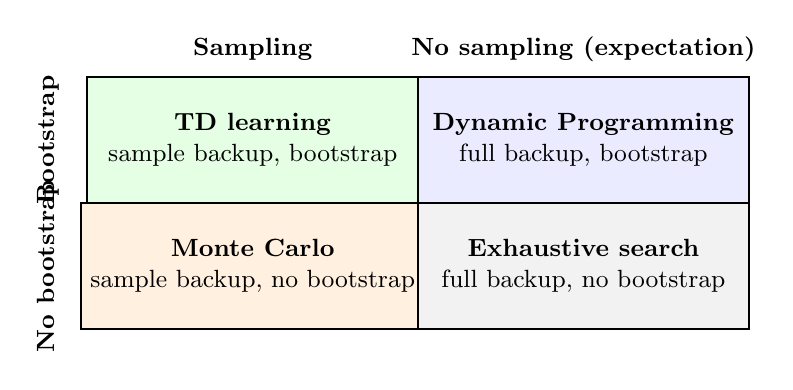
\begin{tikzpicture}[cell/.style={draw, thick, minimum width=4.2cm, minimum height=1.6cm, align=center, font=\small}]
  \node[cell, fill=green!10] (td) at (0,0)     {\textbf{TD learning}\\sample backup, bootstrap};
  \node[cell, fill=blue!8]   (dp) at (4.2,0)   {\textbf{Dynamic Programming}\\full backup, bootstrap};
  \node[cell, fill=orange!12] (mc) at (0,-1.6) {\textbf{Monte Carlo}\\sample backup, no bootstrap};
  \node[cell, fill=gray!10]  (es) at (4.2,-1.6) {\textbf{Exhaustive search}\\full backup, no bootstrap};
  \node[font=\small\bfseries, rotate=90] at (-2.6,0)    {Bootstrap};
  \node[font=\small\bfseries, rotate=90] at (-2.6,-1.6) {No bootstrap};
  \node[font=\small\bfseries] at (0,1.15)   {Sampling};
  \node[font=\small\bfseries] at (4.2,1.15) {No sampling (expectation)};
\end{tikzpicture}
\caption{\emph{Bootstrapping}: the update involves an estimate. \emph{Sampling}: the update uses samples instead of the full expectation.}
\label{fig:unified-view}
\end{figure}

\section{Exploration Strategies (Bandits)}
\begin{table}[H]
\centering
\small
\begin{tabularx}{\textwidth}{@{}l >{\raggedright\arraybackslash}X l >{\raggedright\arraybackslash}X@{}}
\toprule
\textbf{Method} & \textbf{Action selection} & \textbf{Param.} & \textbf{Notes} \\
\midrule
Greedy & $\argmax_a Q_t(a)$ & -- & no exploration, may get stuck on a suboptimal action \\
$\varepsilon$-greedy & greedy w.p.\ $1-\varepsilon$, random w.p.\ $\varepsilon$ & $\varepsilon$ & simple; explores uniformly, also bad actions \\
Optimistic init. & greedy with $Q_1(a)=Q_0$ high & $Q_0$ & only early exploration, not for non-stationary problems \\
UCB & $\argmax_a\bigl[Q_t(a)+c\sqrt{\ln t/N_t(a)}\bigr]$ & $c$ & explores uncertain actions (Hoeffding) \\
Gradient bandit & softmax on $H_t(a)$, updated with baseline $\bar R_t$ & $\alpha$ & learns preferences, not values \\
\bottomrule
\end{tabularx}
\caption{Exploration strategies for the $k$-armed bandit.}
\label{tab:bandits-summary}
\end{table}

\section{Overview of the Algorithms}
\begin{table}[H]
\centering
\small
\begin{tabularx}{\textwidth}{@{}>{\raggedright\arraybackslash}X l c c c l@{}}
\toprule
\textbf{Algorithm} & \textbf{Problem} & \textbf{Model} & \textbf{Bootstrap} & \textbf{Sampling} & \textbf{Policy} \\
\midrule
Iterative Policy Evaluation & Prediction & yes & yes & no & -- \\
Policy Iteration & Control & yes & yes & no & -- \\
Value Iteration & Control & yes & yes & no & -- \\
\midrule
First/Every-visit MC prediction & Prediction & no & no & yes & on \\
MC Exploring Starts & Control & no & no & yes & on \\
On-policy MC control ($\varepsilon$-soft) & Control & no & no & yes & on \\
Off-policy MC prediction (IS) & Prediction & no & no & yes & off \\
\midrule
TD(0) & Prediction & no & yes & yes & on \\
SARSA & Control & no & yes & yes & on \\
Q-learning & Control & no & yes & yes & off \\
Expected SARSA & Control & no & yes & yes & on/off \\
\bottomrule
\end{tabularx}
\caption{Main properties of the algorithms seen in the course.}
\label{tab:algo-overview}
\end{table}

\section{Update Rules}
Almost all the update rules have the form
\[\textit{NewEstimate}\leftarrow\textit{OldEstimate}+\textit{StepSize}\left[\textit{Target}-\textit{OldEstimate}\right]\]
and the algorithms differ in the estimate they update, in the target and in the step-size. In DP the new value replaces the old one (step-size 1).
\begin{table}[H]
\centering
\footnotesize
\renewcommand{\arraystretch}{1.4}
\begin{tabular}{@{}l l l l@{}}
\toprule
\textbf{Algorithm} & \textbf{Estimate} & \textbf{Target} & \textbf{Step-size} \\
\midrule
Sample average (bandits) & $Q(A)$ & $R$ & $1/N(A)$ \\
Constant step-size (bandits) & $Q(A)$ & $R$ & $\alpha$ \\
Iterative Policy Evaluation & $V(s)$ & $\sum_a\pi(a|s)\sum_{s',r}p(s',r|s,a)\left[r+\gamma V(s')\right]$ & 1 \\
Value Iteration & $V(s)$ & $\max_a\sum_{s',r}p(s',r|s,a)\left[r+\gamma V(s')\right]$ & 1 \\
MC prediction & $V(S_t)$ & $G_t$ & $1/N(S_t)$ or $\alpha$ \\
MC control & $Q(S_t,A_t)$ & $G_t$ & $1/N(S_t,A_t)$ \\
Off-policy MC (ordinary IS) & $V(S_t)$ & $\rho_{t:T-1}G_t$ & $1/N(S_t)$ \\
Off-policy MC (weighted IS) & $Q(S_t,A_t)$ & $G_t$ & $W/C(S_t,A_t)$ \\
TD(0) & $V(S_t)$ & $R_{t+1}+\gamma V(S_{t+1})$ & $\alpha$ \\
SARSA & $Q(S_t,A_t)$ & $R_{t+1}+\gamma Q(S_{t+1},A_{t+1})$ & $\alpha$ \\
Q-learning & $Q(S_t,A_t)$ & $R_{t+1}+\gamma\max_aQ(S_{t+1},a)$ & $\alpha$ \\
Expected SARSA & $Q(S_t,A_t)$ & $R_{t+1}+\gamma\sum_a\pi(a|S_{t+1})Q(S_{t+1},a)$ & $\alpha$ \\
\bottomrule
\end{tabular}
\caption{Estimate, target and step-size of the update rules seen in the course.}
\label{tab:update-rules}
\end{table}
Two updates do not follow this scheme: policy improvement, $\pi(s)\leftarrow\argmax_a\sum_{s',r}p(s',r|s,a)\left[r+\gamma V(s')\right]$ (or $\argmax_aQ(s,a)$ in the model-free case), and the gradient bandit, $H_{t+1}(a)=H_t(a)+\alpha(R_t-\bar R_t)\left(\mathds{1}_{a=A_t}-\pi_t(a)\right)$.

\section{Monte Carlo vs.\ TD Learning}
\begin{table}[H]
\centering
\small
\begin{tabularx}{\textwidth}{@{}l >{\raggedright\arraybackslash}X >{\raggedright\arraybackslash}X@{}}
\toprule
 & \textbf{Monte Carlo} & \textbf{TD(0)} \\
\midrule
Target & $G_t$ & $R_{t+1}+\gamma V(S_{t+1})$ \\
Bias / variance & zero bias, high variance & some bias, low variance \\
When it updates & at the end of the episode & after every step (online) \\
Tasks & episodic only & episodic and continuing \\
Initial values & not very sensitive & more sensitive \\
Batch solution & minimum MSE on the observed returns & maximum-likelihood Markov model \\
Markov property & not exploited & exploited (more efficient in Markov environments) \\
\bottomrule
\end{tabularx}
\caption{Comparison between Monte Carlo and TD(0) prediction.}
\label{tab:mc-vs-td}
\end{table}

\section{TD Control: SARSA, Q-learning and Expected SARSA}
\begin{table}[H]
\centering
\footnotesize
\begin{tabularx}{\textwidth}{@{}l >{\raggedright\arraybackslash}X >{\raggedright\arraybackslash}X >{\raggedright\arraybackslash}X@{}}
\toprule
 & \textbf{SARSA} & \textbf{Q-learning} & \textbf{Expected SARSA} \\
\midrule
TD target & $R_{t+1}+\gamma Q(S_{t+1},A_{t+1})$ & $R_{t+1}+\gamma\max_{a'}Q(S_{t+1},a')$ & $R_{t+1}+\gamma\sum_{a'}\pi(a'|S_{t+1})Q(S_{t+1},a')$ \\
Bellman equation & expectation ($q_\pi$) & optimality ($q_*$) & expectation ($q_\pi$) \\
DP counterpart & policy iteration & value iteration & policy iteration \\
On/off-policy & on-policy & off-policy & off-policy (also on-policy) \\
Next action & sampled from $\pi$ & greedy (max) & expectation under $\pi$ \\
Properties & safer path in Cliff Walking, slower in Windy Gridworld & learns $q_*$ directly, usually faster; risky path in Cliff Walking & lower variance, tolerates larger $\alpha$, more computation per step \\
\bottomrule
\end{tabularx}
\caption{Comparison between the TD control algorithms.}
\label{tab:td-control}
\end{table}

\begin{figure}[H]
\centering
\begin{tikzpicture}[
    >={Stealth[length=2.4mm]},
    eq/.style={draw, thick, fill=blue!6, align=center, font=\footnotesize, inner sep=5pt},
    alg/.style={draw, thick, rounded corners, fill=green!8, align=center, font=\footnotesize, inner sep=4pt},
    lab/.style={font=\footnotesize\bfseries}
]
  \node[eq] (be) at (-3.0,0) {Bellman Expectation Equation\\for $q_\pi$};
  \node[eq] (bo) at (3.5,0) {Bellman Optimality Equation\\for $q_*$};
  \node[alg] (sarsa) at (-4.3,-2.0) {\textbf{SARSA} (on-policy)\\[2pt]$R_{t+1}+\gamma Q(S_{t+1},A_{t+1})$};
  \node[alg] (ql) at (3.5,-2.0) {\textbf{Q-learning} (off-policy)\\[2pt]$R_{t+1}+\gamma\max_{a'}Q(S_{t+1},a')$};
  \node[alg] (esarsa) at (-0.6,-3.8) {\textbf{Expected SARSA} (off-policy)\\[2pt]$R_{t+1}+\gamma\sum_{a'}\pi(a'|S_{t+1})Q(S_{t+1},a')$};
  \draw[->, thick] (be) -- node[font=\footnotesize, left] {sample $A_{t+1}$} (sarsa);
  \draw[->, thick] (be) -- node[font=\footnotesize, right] {expectation} (esarsa);
  \draw[->, thick] (bo) -- node[font=\footnotesize, right] {max} (ql);
\end{tikzpicture}
\caption{TD control algorithms as sample-based versions of the Bellman equations (policy iteration for SARSA and Expected SARSA, value iteration for Q-learning).}
\label{fig:td-control-bellman}
\end{figure}

\section{Pseudocode of All the Algorithms}
\label{sec:all-pseudocode}

The table below collects the pseudocode of every algorithm seen in the course, grouped by family, so that they can be compared side by side. Notation: $\mathcal{S}^+$ is the set of states including the terminal one, $\leftarrow$ is an assignment, and ties in $\arg\max$ are broken randomly unless stated otherwise. Double Q-learning (Section 6.7 of the book) is reported for completeness only, since it is not part of the exam program.

% indentation and cell helpers used only in this table
\newcommand{\Ii}{\hspace*{1.2em}}
\newcommand{\Iii}{\hspace*{2.4em}}
\newcommand{\Iiii}{\hspace*{3.6em}}
\newcommand{\pc}[1]{\begin{minipage}[t]{\linewidth}\raggedright #1\par\vspace{3pt}\end{minipage}}
\newcommand{\algfam}[1]{\multicolumn{2}{@{}l@{}}{\cellcolor{blue!8}\rule{0pt}{2.6ex}\textbf{#1}}\\*\midrule}
\newcommand{\algname}[2]{\pc{\textbf{#1}\\[2pt]\textit{#2}}}

{\footnotesize
\renewcommand{\arraystretch}{1.1}
\begin{longtable}{@{}p{3.1cm}p{\dimexpr\textwidth-3.1cm-2\tabcolsep\relax}@{}}
\caption{Pseudocode of all the algorithms of the course.}\label{tab:all-pseudocode}\\
\toprule
\textbf{Algorithm} & \textbf{Pseudocode} \\
\midrule
\endfirsthead
\toprule
\textbf{Algorithm} & \textbf{Pseudocode} \\
\midrule
\endhead
\bottomrule
\endfoot
%-------------------------------------------------------------
\algfam{Multi-armed bandits}
\algname{1. Simple bandit ($\varepsilon$-greedy, sample average)}{Nonassociative, action-value method} &
\pc{Parameter: $\varepsilon \ge 0$\\
Initialize, for $a = 1,\dots,k$: $Q(a) \leftarrow 0$, $N(a) \leftarrow 0$\\
Loop forever:\\
\Ii$A \leftarrow \begin{cases} \arg\max_a Q(a) & \text{with probability } 1-\varepsilon\\ \text{a random action} & \text{with probability } \varepsilon\end{cases}$\\
\Ii$R \leftarrow \mathit{bandit}(A)$\\
\Ii$N(A) \leftarrow N(A) + 1$\\
\Ii$Q(A) \leftarrow Q(A) + \frac{1}{N(A)}\bigl[R - Q(A)\bigr]$} \\
\midrule
\algname{2. Constant step-size bandit}{Nonstationary problems (exponential recency-weighted average)} &
\pc{As algorithm 1, with parameter $\alpha \in (0,1]$ and the last update replaced by:\\
\Ii$Q(A) \leftarrow Q(A) + \alpha\bigl[R - Q(A)\bigr]$} \\
\midrule
\algname{3. Optimistic initial values}{Exploration through initialization} &
\pc{As algorithm 1 (or 2) with $\varepsilon = 0$ (purely greedy) and optimistic initialization:\\
\Ii$Q(a) \leftarrow Q_0$ for all $a$, with $Q_0$ much larger than any expected reward (e.g.\ $Q_0 = +5$)\\
Every selected action ``disappoints'', so all actions are tried in the first steps.} \\
\midrule
\algname{4. Upper Confidence Bound (UCB)}{Exploration based on uncertainty} &
\pc{Parameter: $c > 0$\\
Initialize, for $a = 1,\dots,k$: $Q(a) \leftarrow 0$, $N(a) \leftarrow 0$; $t \leftarrow 0$\\
Loop forever:\\
\Ii$t \leftarrow t + 1$\\
\Ii If some $a$ has $N(a) = 0$: $A \leftarrow a$ (maximizing action)\\
\Ii Else: $A \leftarrow \arg\max_a \Bigl[Q(a) + c\sqrt{\frac{\ln t}{N(a)}}\Bigr]$\\
\Ii$R \leftarrow \mathit{bandit}(A)$\\
\Ii$N(A) \leftarrow N(A) + 1$\\
\Ii$Q(A) \leftarrow Q(A) + \frac{1}{N(A)}\bigl[R - Q(A)\bigr]$} \\
\midrule
\algname{5. Gradient bandit}{Preferences + softmax, stochastic gradient ascent} &
\pc{Parameter: $\alpha > 0$\\
Initialize, for $a = 1,\dots,k$: $H(a) \leftarrow 0$; $\bar{R} \leftarrow 0$; $t \leftarrow 0$\\
Loop forever:\\
\Ii$t \leftarrow t + 1$\\
\Ii$\pi(a) \leftarrow \dfrac{e^{H(a)}}{\sum_{b=1}^{k} e^{H(b)}}$ for all $a$\\
\Ii$A \sim \pi$;\quad $R \leftarrow \mathit{bandit}(A)$\\
\Ii$H(A) \leftarrow H(A) + \alpha (R - \bar{R})\bigl(1 - \pi(A)\bigr)$\\
\Ii$H(a) \leftarrow H(a) - \alpha (R - \bar{R})\,\pi(a)$ for all $a \neq A$\\
\Ii$\bar{R} \leftarrow \bar{R} + \frac{1}{t}(R - \bar{R})$\\(the baseline is updated after $H$: it averages the rewards up to but not including $t$)} \\
\pagebreak
%-------------------------------------------------------------
\algfam{Dynamic Programming (model $p(s',r\mid s,a)$ known)}
\algname{6. Iterative policy evaluation (synchronous)}{Prediction, two arrays} &
\pc{Input: $\pi$; parameter: threshold $\theta > 0$\\
Initialize $V(s)$ arbitrarily for all $s \in \mathcal{S}^+$, $V(\text{terminal}) = 0$\\
Loop:\\
\Ii For each $s \in \mathcal{S}$:\\
\Iii$V_{\text{new}}(s) \leftarrow \sum_a \pi(a\mid s) \sum_{s',r} p(s',r\mid s,a)\bigl[r + \gamma V(s')\bigr]$\\
\Ii$\Delta \leftarrow \max_s |V_{\text{new}}(s) - V(s)|$\\
\Ii$V \leftarrow V_{\text{new}}$\\
until $\Delta < \theta$} \\
\midrule
\algname{7. Iterative policy evaluation (in-place)}{Prediction, one array, usually faster} &
\pc{Input: $\pi$; parameter: threshold $\theta > 0$\\
Initialize $V(s)$ arbitrarily for all $s \in \mathcal{S}^+$, $V(\text{terminal}) = 0$\\
Loop:\\
\Ii$\Delta \leftarrow 0$\\
\Ii For each $s \in \mathcal{S}$:\\
\Iii$v \leftarrow V(s)$\\
\Iii$V(s) \leftarrow \sum_a \pi(a\mid s) \sum_{s',r} p(s',r\mid s,a)\bigl[r + \gamma V(s')\bigr]$\\
\Iii$\Delta \leftarrow \max(\Delta, |v - V(s)|)$\\
until $\Delta < \theta$} \\
\midrule
\algname{8. Policy iteration}{Control: full evaluation + greedy improvement} &
\pc{1. Initialization: $V(s) \in \mathbb{R}$ and $\pi(s) \in \mathcal{A}(s)$ arbitrarily for all $s \in \mathcal{S}$; $V(\text{terminal}) = 0$\\
2. Policy evaluation: run algorithm 7 on the current $\pi$ (deterministic: $V(s) \leftarrow \sum_{s',r} p(s',r\mid s,\pi(s))[r + \gamma V(s')]$)\\
3. Policy improvement:\\
\Ii$\mathit{policy\text{-}stable} \leftarrow \mathit{true}$\\
\Ii For each $s \in \mathcal{S}$:\\
\Iii$\mathit{old} \leftarrow \pi(s)$\\
\Iii$\pi(s) \leftarrow \arg\max_a \sum_{s',r} p(s',r\mid s,a)\bigl[r + \gamma V(s')\bigr]$\\
\Iii If $\mathit{old} \neq \pi(s)$: $\mathit{policy\text{-}stable} \leftarrow \mathit{false}$\\
\Ii If $\mathit{policy\text{-}stable}$: stop and return $V \approx v_*$, $\pi \approx \pi_*$; else go to 2} \\
\midrule
\algname{9. Value iteration}{Control: one sweep of evaluation with max} &
\pc{Parameter: threshold $\theta > 0$\\
Initialize $V(s)$ arbitrarily for all $s \in \mathcal{S}^+$, $V(\text{terminal}) = 0$\\
Loop:\\
\Ii$\Delta \leftarrow 0$\\
\Ii For each $s \in \mathcal{S}$:\\
\Iii$v \leftarrow V(s)$\\
\Iii$V(s) \leftarrow \max_a \sum_{s',r} p(s',r\mid s,a)\bigl[r + \gamma V(s')\bigr]$\\
\Iii$\Delta \leftarrow \max(\Delta, |v - V(s)|)$\\
until $\Delta < \theta$\\
Output the deterministic policy $\pi \approx \pi_*$: $\pi(s) = \arg\max_a \sum_{s',r} p(s',r\mid s,a)\bigl[r + \gamma V(s')\bigr]$} \\
\midrule
\algname{10. Asynchronous DP}{Control, states updated in any order} &
\pc{Initialize $V(s)$ arbitrarily, $V(\text{terminal}) = 0$\\
Loop:\\
\Ii Pick a state $s$ (any order: random, along real trajectories, by priority as in prioritized sweeping, \dots)\\
\Ii$V(s) \leftarrow \max_a \sum_{s',r} p(s',r\mid s,a)\bigl[r + \gamma V(s')\bigr]$\\
until convergence (every state must keep being selected, i.e.\ infinitely often)} \\
\pagebreak
%-------------------------------------------------------------
\algfam{Monte Carlo methods (model-free, episodic tasks)}
\algname{11. First-visit MC prediction}{Prediction of $V \approx v_\pi$} &
\pc{Input: $\pi$\\
Initialize: $V(s)$ arbitrarily, $\mathit{Returns}(s) \leftarrow$ empty list, for all $s \in \mathcal{S}$\\
Loop forever (for each episode):\\
\Ii Generate an episode following $\pi$:\\\Iii$S_0, A_0, R_1, \dots, S_{T-1}, A_{T-1}, R_T$\\
\Ii$G \leftarrow 0$\\
\Ii Loop for $t = T-1, T-2, \dots, 0$:\\
\Iii$G \leftarrow \gamma G + R_{t+1}$\\
\Iii Unless $S_t$ appears in $S_0, \dots, S_{t-1}$:\\
\Iiii Append $G$ to $\mathit{Returns}(S_t)$\\
\Iiii$V(S_t) \leftarrow \mathrm{average}(\mathit{Returns}(S_t))$} \\
\midrule
\algname{12. Every-visit MC prediction (incremental)}{Prediction of $V \approx v_\pi$} &
\pc{As algorithm 11, without the ``unless'' check (every occurrence of $S_t$ is used), and with the incremental mean instead of the list:\\
\Ii$N(S_t) \leftarrow N(S_t) + 1$\\
\Ii$V(S_t) \leftarrow V(S_t) + \frac{1}{N(S_t)}\bigl[G - V(S_t)\bigr]$\quad (or $\alpha$ instead of $\frac{1}{N}$ for nonstationary problems)} \\
\midrule
\algname{13. Monte Carlo ES (Exploring Starts)}{Control, $\pi \approx \pi_*$} &
\pc{Initialize: $\pi(s) \in \mathcal{A}(s)$, $Q(s,a) \in \mathbb{R}$ arbitrarily, $\mathit{Returns}(s,a) \leftarrow$ empty list\\
Loop forever (for each episode):\\
\Ii Choose $S_0 \in \mathcal{S}$, $A_0 \in \mathcal{A}(S_0)$ randomly, so that all pairs have probability $> 0$\\
\Ii Generate an episode from $S_0, A_0$ following $\pi$:\\\Iii$S_0, A_0, R_1, \dots, S_{T-1}, A_{T-1}, R_T$\\
\Ii$G \leftarrow 0$\\
\Ii Loop for $t = T-1, T-2, \dots, 0$:\\
\Iii$G \leftarrow \gamma G + R_{t+1}$\\
\Iii Unless the pair $S_t, A_t$ appears in $S_0, A_0, \dots, S_{t-1}, A_{t-1}$:\\
\Iiii Append $G$ to $\mathit{Returns}(S_t, A_t)$\\
\Iiii$Q(S_t, A_t) \leftarrow \mathrm{average}(\mathit{Returns}(S_t, A_t))$\\
\Iiii$\pi(S_t) \leftarrow \arg\max_a Q(S_t, a)$} \\
\midrule
\algname{14. On-policy first-visit MC control}{Control with $\varepsilon$-soft policies (no exploring starts)} &
\pc{Parameter: small $\varepsilon > 0$\\
Initialize: $\pi \leftarrow$ an arbitrary $\varepsilon$-soft policy; $Q(s,a)$ arbitrarily; $\mathit{Returns}(s,a) \leftarrow$ empty list\\
Loop forever (for each episode):\\
\Ii Generate an episode following $\pi$:\\\Iii$S_0, A_0, R_1, \dots, S_{T-1}, A_{T-1}, R_T$\\
\Ii$G \leftarrow 0$\\
\Ii Loop for $t = T-1, T-2, \dots, 0$:\\
\Iii$G \leftarrow \gamma G + R_{t+1}$\\
\Iii Unless the pair $S_t, A_t$ appears in $S_0, A_0, \dots, S_{t-1}, A_{t-1}$:\\
\Iiii Append $G$ to $\mathit{Returns}(S_t, A_t)$\\
\Iiii$Q(S_t, A_t) \leftarrow \mathrm{average}(\mathit{Returns}(S_t, A_t))$\\
\Iiii$A^* \leftarrow \arg\max_a Q(S_t, a)$\\
\Iiii For all $a \in \mathcal{A}(S_t)$:\\
\Iiii\Ii$\pi(a\mid S_t) \leftarrow \begin{cases} 1 - \varepsilon + \varepsilon/|\mathcal{A}(S_t)| & \text{if } a = A^*\\ \varepsilon/|\mathcal{A}(S_t)| & \text{if } a \neq A^*\end{cases}$} \\
\midrule
\algname{15. Off-policy MC prediction, ordinary IS}{Prediction of $V \approx v_\pi$ (version of the slides)} &
\pc{Input: target policy $\pi$, behavior policy $b$ with coverage of $\pi$\\
Initialize: $V(s)$ arbitrarily, $V(\text{terminal}) = 0$, $N(s) \leftarrow 0$\\
Loop forever (for each episode):\\
\Ii Generate an episode following $b$:\\\Iii$S_0, A_0, R_1, \dots, S_{T-1}, A_{T-1}, R_T$\\
\Ii$G \leftarrow 0$, $W \leftarrow 1$\\
\Ii Loop for $t = T-1, T-2, \dots, 0$, while $W \neq 0$:\\
\Iii$G \leftarrow \gamma G + R_{t+1}$\\
\Iii$W \leftarrow W \frac{\pi(A_t\mid S_t)}{b(A_t\mid S_t)}$\quad (before the update: $A_t$ was chosen by $b$)\\
\Iii$N(S_t) \leftarrow N(S_t) + 1$\\
\Iii$V(S_t) \leftarrow V(S_t) + \frac{1}{N(S_t)}\bigl[W G - V(S_t)\bigr]$} \\
\midrule
\algname{16. Off-policy MC prediction, weighted IS}{Prediction of $Q \approx q_\pi$} &
\pc{Input: an arbitrary target policy $\pi$\\
Initialize, for all $s, a$: $Q(s,a)$ arbitrarily, $C(s,a) \leftarrow 0$\\
Loop forever (for each episode):\\
\Ii$b \leftarrow$ any policy with coverage of $\pi$\\
\Ii Generate an episode following $b$:\\\Iii$S_0, A_0, R_1, \dots, S_{T-1}, A_{T-1}, R_T$\\
\Ii$G \leftarrow 0$, $W \leftarrow 1$\\
\Ii Loop for $t = T-1, T-2, \dots, 0$, while $W \neq 0$:\\
\Iii$G \leftarrow \gamma G + R_{t+1}$\\
\Iii$C(S_t,A_t) \leftarrow C(S_t,A_t) + W$\\
\Iii$Q(S_t,A_t) \leftarrow Q(S_t,A_t) + \frac{W}{C(S_t,A_t)}\bigl[G - Q(S_t,A_t)\bigr]$\\
\Iii$W \leftarrow W \frac{\pi(A_t\mid S_t)}{b(A_t\mid S_t)}$\quad (after the update: $A_t$ is given)} \\
\midrule
\algname{17. Off-policy MC control}{Control, weighted IS, $\pi \approx \pi_*$} &
\pc{Initialize, for all $s, a$: $Q(s,a)$ arbitrarily, $C(s,a) \leftarrow 0$, $\pi(s) \leftarrow \arg\max_a Q(s,a)$ (ties broken consistently)\\
Loop forever (for each episode):\\
\Ii$b \leftarrow$ any soft policy\\
\Ii Generate an episode following $b$:\\\Iii$S_0, A_0, R_1, \dots, S_{T-1}, A_{T-1}, R_T$\\
\Ii$G \leftarrow 0$, $W \leftarrow 1$\\
\Ii Loop for $t = T-1, T-2, \dots, 0$:\\
\Iii$G \leftarrow \gamma G + R_{t+1}$\\
\Iii$C(S_t,A_t) \leftarrow C(S_t,A_t) + W$\\
\Iii$Q(S_t,A_t) \leftarrow Q(S_t,A_t) + \frac{W}{C(S_t,A_t)}\bigl[G - Q(S_t,A_t)\bigr]$\\
\Iii$\pi(S_t) \leftarrow \arg\max_a Q(S_t,a)$\\
\Iii If $A_t \neq \pi(S_t)$: exit the inner loop (go to the next episode)\\
\Iii$W \leftarrow W \frac{1}{b(A_t\mid S_t)}$\quad ($\pi$ is greedy, so $\pi(A_t\mid S_t) = 1$)} \\
\pagebreak
%-------------------------------------------------------------
\algfam{Temporal-Difference learning (model-free, bootstrapping)}
\algname{18. Tabular TD(0)}{Prediction of $V \approx v_\pi$} &
\pc{Input: $\pi$; parameter: step size $\alpha \in (0,1]$\\
Initialize $V(s)$ arbitrarily for all $s \in \mathcal{S}^+$, $V(\text{terminal}) = 0$\\
Loop for each episode:\\
\Ii Initialize $S$\\
\Ii Loop for each step of episode:\\
\Iii$A \leftarrow$ action given by $\pi$ for $S$\\
\Iii Take action $A$, observe $R, S'$\\
\Iii$V(S) \leftarrow V(S) + \alpha\bigl[R + \gamma V(S') - V(S)\bigr]$\\
\Iii$S \leftarrow S'$\\
\Ii until $S$ is terminal} \\
\midrule
\algname{19. Batch MC / batch TD(0)}{Prediction with a finite amount of experience} &
\pc{Given a finite set of episodes (or transitions):\\
Loop until $V$ converges:\\
\Ii For each time step $t$ of all the episodes: compute the increment\\
\Iii MC: $\Delta V(S_t) \mathrel{+}= \alpha\bigl[G_t - V(S_t)\bigr]$\\
\Iii TD(0): $\Delta V(S_t) \mathrel{+}= \alpha\bigl[R_{t+1} + \gamma V(S_{t+1}) - V(S_t)\bigr]$\\
\Ii Apply all the increments at once: $V \leftarrow V + \Delta V$, then reset $\Delta V \leftarrow 0$\\
Batch MC converges to the minimum MSE on the training returns; batch TD(0) to the certainty-equivalence estimate (maximum-likelihood model of the MDP).} \\
\midrule
\algname{20. SARSA}{On-policy TD control, $Q \approx q_*$} &
\pc{Parameters: step size $\alpha \in (0,1]$, small $\varepsilon > 0$\\
Initialize $Q(s,a)$ arbitrarily for all $s \in \mathcal{S}^+, a \in \mathcal{A}(s)$, $Q(\text{terminal},\cdot) = 0$\\
Loop for each episode:\\
\Ii Initialize $S$\\
\Ii Choose $A$ from $S$ using the $\varepsilon$-greedy policy derived from $Q$\\
\Ii Loop for each step of episode:\\
\Iii Take action $A$, observe $R, S'$\\
\Iii Choose $A'$ from $S'$ using the $\varepsilon$-greedy policy derived from $Q$\\
\Iii$Q(S,A) \leftarrow Q(S,A) + \alpha\bigl[R + \gamma Q(S',A') - Q(S,A)\bigr]$\\
\Iii$S \leftarrow S'$;\quad $A \leftarrow A'$\\
\Ii until $S$ is terminal} \\
\midrule
\algname{21. Q-learning}{Off-policy TD control, $\pi \approx \pi_*$} &
\pc{Parameters: step size $\alpha \in (0,1]$, small $\varepsilon > 0$\\
Initialize $Q(s,a)$ arbitrarily for all $s \in \mathcal{S}^+, a \in \mathcal{A}(s)$, $Q(\text{terminal},\cdot) = 0$\\
Loop for each episode:\\
\Ii Initialize $S$\\
\Ii Loop for each step of episode:\\
\Iii Choose $A$ from $S$ using the $\varepsilon$-greedy policy derived from $Q$\\
\Iii Take action $A$, observe $R, S'$\\
\Iii$Q(S,A) \leftarrow Q(S,A) + \alpha\bigl[R + \gamma \max_a Q(S',a) - Q(S,A)\bigr]$\\
\Iii$S \leftarrow S'$\\
\Ii until $S$ is terminal} \\
\midrule
\algname{22. Expected SARSA}{TD control, off-policy (also on-policy), $Q \approx q_\pi$ or $q_*$} &
\pc{Parameters: step size $\alpha \in (0,1]$, small $\varepsilon > 0$; target policy $\pi$ (e.g.\ $\varepsilon$-greedy or greedy w.r.t.\ $Q$)\\
Initialize $Q(s,a)$ arbitrarily for all $s \in \mathcal{S}^+, a \in \mathcal{A}(s)$, $Q(\text{terminal},\cdot) = 0$\\
Loop for each episode:\\
\Ii Initialize $S$\\
\Ii Loop for each step of episode:\\
\Iii Choose $A$ from $S$ using the behavior policy (e.g.\ $\varepsilon$-greedy in $Q$)\\
\Iii Take action $A$, observe $R, S'$\\
\Iii$Q(S,A) \leftarrow Q(S,A)$\\
\Iiii$\quad + \alpha\bigl[R + \gamma \sum_a \pi(a\mid S')\, Q(S',a) - Q(S,A)\bigr]$\\
\Iii$S \leftarrow S'$\\
\Ii until $S$ is terminal\\
If $\pi$ is greedy, Expected SARSA reduces to Q-learning.} \\
\midrule
\algname{23. Double Q-learning}{Off-policy TD control, avoids maximization bias (Sec.\ 6.7, not in the exam)} &
\pc{Parameters: step size $\alpha \in (0,1]$, small $\varepsilon > 0$\\
Initialize $Q_1(s,a)$, $Q_2(s,a)$ arbitrarily, $Q_i(\text{terminal},\cdot) = 0$\\
Loop for each episode:\\
\Ii Initialize $S$\\
\Ii Loop for each step of episode:\\
\Iii Choose $A$ from $S$ using the policy $\varepsilon$-greedy in $Q_1 + Q_2$\\
\Iii Take action $A$, observe $R, S'$\\
\Iii With probability $0.5$:\\
\Iiii$Q_1(S,A) \leftarrow Q_1(S,A)$\\
\Iiii\Ii$\quad + \alpha\bigl[R + \gamma Q_2\bigl(S', \arg\max_a Q_1(S',a)\bigr) - Q_1(S,A)\bigr]$\\
\Iii else:\\
\Iiii$Q_2(S,A) \leftarrow Q_2(S,A)$\\
\Iiii\Ii$\quad + \alpha\bigl[R + \gamma Q_1\bigl(S', \arg\max_a Q_2(S',a)\bigr) - Q_2(S,A)\bigr]$\\
\Iii$S \leftarrow S'$\\
\Ii until $S$ is terminal} \\
\end{longtable}
}
